\documentclass[12pt]{article}
\usepackage[margin=2.5cm]{geometry}
\usepackage{enumerate}
\usepackage{amsfonts}
\usepackage{amsmath}
\usepackage{fancyhdr}
\usepackage{amsmath}
\usepackage{amssymb}
\usepackage{amsthm}
\usepackage{mdframed}
\usepackage{graphicx}
\usepackage{subcaption}
\usepackage{adjustbox}
\usepackage{listings}
\usepackage{xcolor}
\usepackage{courier}
\usepackage[utf]{kotex}
\usepackage{hyperref}

\definecolor{codegreen}{rgb}{0,0.6,0}
\definecolor{codegray}{rgb}{0.5,0.5,0.5}
\definecolor{codepurple}{rgb}{0.58,0,0.82}
\definecolor{backcolour}{rgb}{0.95,0.95,0.92}

\lstdefinestyle{mystyle}{
    backgroundcolor=\color{backcolour},
    commentstyle=\color{codegreen},
    keywordstyle=\color{magenta},
    numberstyle=\tiny\color{codegray},
    stringstyle=\color{codepurple},
    basicstyle=\ttfamily\footnotesize,
    breakatwhitespace=false,
    breaklines=true,
    captionpos=b,
    keepspaces=true,
    numbers=left,
    numbersep=5pt,
    showspaces=false,
    showstringspaces=false,
    showtabs=false,
    tabsize=1
}

\lstset{style=mystyle}

\pagestyle{fancy}
\renewcommand{\headrulewidth}{0.4pt}
\lhead{CSC 369}
\rhead{Worksheet 7 Solution}

\begin{document}
\title{CSC 369 Worksheet 7 Solution}

\maketitle

\bigskip

\begin{enumerate}[1.]
    \item

    First, I need to run the program with seeds 1,2, and 3, and compute whether
    each virtual address generated by the process is in or out of bounds.

    \bigskip

    By running the following commands, we see the corresponding base bounds register
    information (see images under each command).

    \begin{itemize}
        \item \texttt{./relocation.py -s 1}

        \begin{center}
        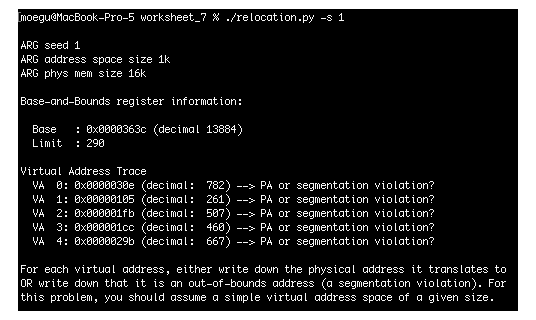
\includegraphics[width=0.8\linewidth]{images/worksheet_7_solution_1.png}
        \end{center}

        \bigskip

        Here, the following is inbound:

        \begin{itemize}
            \item VA  1: 0x00000105 (decimal:  261) --> PA 0x00003741 (decimal 14145)
        \end{itemize}

        \bigskip

        and the following is out of bound:

        \begin{itemize}
            \item VA  0: 0x0000030e (decimal:  782)
            \item VA  2: 0x000001fb (decimal:  507)
            \item VA  3: 0x000001cc (decimal:  460)
            \item VA  4: 0x0000029b (decimal:  667)
        \end{itemize}

        \item \texttt{./relocation.py -s 2}

        \begin{center}
        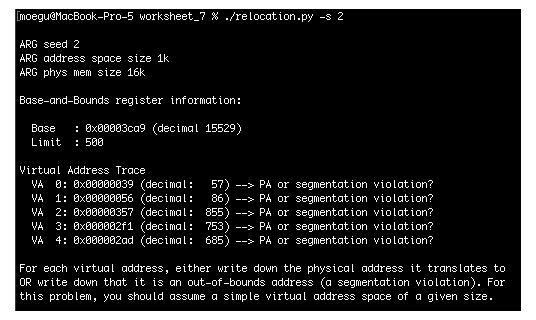
\includegraphics[width=0.8\linewidth]{images/worksheet_7_solution_2.png}
        \end{center}

        \bigskip

        Here, the following is inbound:

        \begin{itemize}
            \item VA  0: 0x00000039 (decimal:   57) --> PA 0x00003CE2 (decimal 15586)
            \item VA  1: 0x00000056 (decimal:   86) --> PA 0x00003CFF (decimal 15615)
        \end{itemize}

        \bigskip

        and the following is out of bound:

        \begin{itemize}
            \item VA  2: 0x00000357 (decimal:  855)
            \item VA  3: 0x000002f1 (decimal:  753)
            \item VA  4: 0x000002ad (decimal:  685)
        \end{itemize}


        \item \texttt{./relocation.py -s 3}

        \begin{center}
        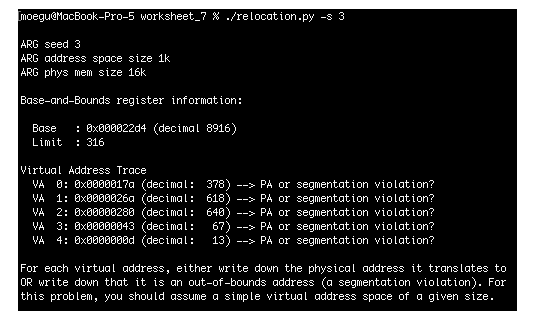
\includegraphics[width=0.8\linewidth]{images/worksheet_7_solution_3.png}
        \end{center}

        \bigskip

        Here, the following is inbound:

        \begin{itemize}
            \item VA  3: 0x00000043 (decimal:   67) --> PA 0x00002317 (decimal 8983)
            \item VA  4: 0x0000000d (decimal:   13) --> PA 0x000022E1 (decimal 8929)
        \end{itemize}

        \bigskip

        and the following is out of bound:

        \begin{itemize}
            \item VA  0: 0x0000017a (decimal:  378)
            \item VA  1: 0x0000026a (decimal:  618)
            \item VA  2: 0x00000280 (decimal:  640)
        \end{itemize}
    \end{itemize}



    \bigskip

    Second, for the ones that are in bounds, I need to calculate the translation.

    \underline{\textbf{Notes}}

    \begin{enumerate}[1.]
        \item Decimal to hexadecimal link \href{https://www.binaryhexconverter.com/decimal-to-hex-converter}{here}
        \item The prefix \texttt{0x} in \texttt{0x00003ca9} is to indicate that the number is written in hex
        \item Simulation is run with command
        \item Reality $\to$ many programs share memory at the same time
        \item Virtualization $\to$ creates illution that program has its own private
        memory, where its own code and data inside
        \item Virtualization allows us turn into something useful, powerful and easy to use
        \item \textbf{Dynamic (Hardware-based) Relocation}

        \begin{itemize}
            \item
        \end{itemize}
    \end{enumerate}
\end{enumerate}

\end{document}